\documentclass[journal]{IEEEtran}
\usepackage{cite}
\usepackage{amsmath,amssymb,amsfonts}
\usepackage{graphicx}
\usepackage{booktabs}
\usepackage{tikz}
\usetikzlibrary{arrows.meta,positioning,calc,fit,backgrounds}
\usepackage{textcomp}
\usepackage[hidelinks]{hyperref}
\newcommand{\gapLoneDzero}{10.2}
\newcommand{\collLoneDzero}{0}
\newcommand{\vminLoneDzero}{13.0}
\newcommand{\hwLoneDzero}{0.78}
\newcommand{\revnLoneDzero}{0}
\newcommand{\minwLoneDzero}{1.00}
\newcommand{\revtLoneDzero}{--}
\newcommand{\detLoneDzero}{--}
\newcommand{\gapLoneDone}{10.2}
\newcommand{\collLoneDone}{0}
\newcommand{\vminLoneDone}{13.0}
\newcommand{\hwLoneDone}{0.78}
\newcommand{\revnLoneDone}{0}
\newcommand{\minwLoneDone}{1.00}
\newcommand{\revtLoneDone}{--}
\newcommand{\detLoneDone}{--}
\newcommand{\gapLoneDtwo}{10.2}
\newcommand{\collLoneDtwo}{0}
\newcommand{\vminLoneDtwo}{13.0}
\newcommand{\hwLoneDtwo}{0.78}
\newcommand{\revnLoneDtwo}{0}
\newcommand{\minwLoneDtwo}{1.00}
\newcommand{\revtLoneDtwo}{--}
\newcommand{\detLoneDtwo}{--}
\newcommand{\gapLoneDtwob}{10.2}
\newcommand{\collLoneDtwob}{0}
\newcommand{\vminLoneDtwob}{13.0}
\newcommand{\hwLoneDtwob}{0.78}
\newcommand{\revnLoneDtwob}{0}
\newcommand{\minwLoneDtwob}{1.00}
\newcommand{\revtLoneDtwob}{--}
\newcommand{\detLoneDtwob}{--}
\newcommand{\gapLoneCA}{10.2}
\newcommand{\collLoneCA}{0}
\newcommand{\vminLoneCA}{13.0}
\newcommand{\hwLoneCA}{0.78}
\newcommand{\revnLoneCA}{0}
\newcommand{\minwLoneCA}{1.00}
\newcommand{\revtLoneCA}{--}
\newcommand{\detLoneCA}{--}
\newcommand{\gapLoneCAnr}{10.2}
\newcommand{\collLoneCAnr}{0}
\newcommand{\vminLoneCAnr}{13.0}
\newcommand{\hwLoneCAnr}{0.78}
\newcommand{\revnLoneCAnr}{0}
\newcommand{\minwLoneCAnr}{1.00}
\newcommand{\revtLoneCAnr}{--}
\newcommand{\detLoneCAnr}{--}
\newcommand{\gapLoneCAfh}{10.2}
\newcommand{\collLoneCAfh}{0}
\newcommand{\vminLoneCAfh}{13.0}
\newcommand{\hwLoneCAfh}{0.78}
\newcommand{\revnLoneCAfh}{0}
\newcommand{\minwLoneCAfh}{1.00}
\newcommand{\revtLoneCAfh}{--}
\newcommand{\detLoneCAfh}{--}
\newcommand{\gapLtwoDzero}{1.3}
\newcommand{\collLtwoDzero}{0}
\newcommand{\vminLtwoDzero}{2.7}
\newcommand{\hwLtwoDzero}{0.85}
\newcommand{\revnLtwoDzero}{0}
\newcommand{\minwLtwoDzero}{1.00}
\newcommand{\revtLtwoDzero}{--}
\newcommand{\detLtwoDzero}{--}
\newcommand{\gapLtwoDone}{1.3}
\newcommand{\collLtwoDone}{0}
\newcommand{\vminLtwoDone}{2.7}
\newcommand{\hwLtwoDone}{0.85}
\newcommand{\revnLtwoDone}{0}
\newcommand{\minwLtwoDone}{1.00}
\newcommand{\revtLtwoDone}{--}
\newcommand{\detLtwoDone}{--}
\newcommand{\gapLtwoDtwo}{$-$4.2}
\newcommand{\collLtwoDtwo}{20}
\newcommand{\vminLtwoDtwo}{1.8}
\newcommand{\hwLtwoDtwo}{0.86}
\newcommand{\revnLtwoDtwo}{0}
\newcommand{\minwLtwoDtwo}{1.00}
\newcommand{\revtLtwoDtwo}{--}
\newcommand{\detLtwoDtwo}{--}
\newcommand{\gapLtwoDtwob}{$-$4.1}
\newcommand{\collLtwoDtwob}{20}
\newcommand{\vminLtwoDtwob}{1.7}
\newcommand{\hwLtwoDtwob}{0.86}
\newcommand{\revnLtwoDtwob}{0}
\newcommand{\minwLtwoDtwob}{1.00}
\newcommand{\revtLtwoDtwob}{--}
\newcommand{\detLtwoDtwob}{--}
\newcommand{\gapLtwoCA}{1.2}
\newcommand{\collLtwoCA}{0}
\newcommand{\vminLtwoCA}{2.7}
\newcommand{\hwLtwoCA}{0.85}
\newcommand{\revnLtwoCA}{0}
\newcommand{\minwLtwoCA}{0.97}
\newcommand{\revtLtwoCA}{--}
\newcommand{\detLtwoCA}{--}
\newcommand{\gapLtwoCAnr}{1.2}
\newcommand{\collLtwoCAnr}{0}
\newcommand{\vminLtwoCAnr}{2.7}
\newcommand{\hwLtwoCAnr}{0.85}
\newcommand{\revnLtwoCAnr}{0}
\newcommand{\minwLtwoCAnr}{0.97}
\newcommand{\revtLtwoCAnr}{--}
\newcommand{\detLtwoCAnr}{--}
\newcommand{\gapLtwoCAfh}{1.2}
\newcommand{\collLtwoCAfh}{0}
\newcommand{\vminLtwoCAfh}{2.7}
\newcommand{\hwLtwoCAfh}{0.85}
\newcommand{\revnLtwoCAfh}{0}
\newcommand{\minwLtwoCAfh}{0.97}
\newcommand{\revtLtwoCAfh}{--}
\newcommand{\detLtwoCAfh}{--}
\newcommand{\gapLthreeDzero}{6.3}
\newcommand{\collLthreeDzero}{0}
\newcommand{\vminLthreeDzero}{6.9}
\newcommand{\hwLthreeDzero}{0.81}
\newcommand{\revnLthreeDzero}{0}
\newcommand{\minwLthreeDzero}{1.00}
\newcommand{\revtLthreeDzero}{--}
\newcommand{\detLthreeDzero}{--}
\newcommand{\gapLthreeDone}{6.3}
\newcommand{\collLthreeDone}{0}
\newcommand{\vminLthreeDone}{6.9}
\newcommand{\hwLthreeDone}{0.81}
\newcommand{\revnLthreeDone}{0}
\newcommand{\minwLthreeDone}{1.00}
\newcommand{\revtLthreeDone}{--}
\newcommand{\detLthreeDone}{--}
\newcommand{\gapLthreeDtwo}{6.3}
\newcommand{\collLthreeDtwo}{0}
\newcommand{\vminLthreeDtwo}{6.9}
\newcommand{\hwLthreeDtwo}{0.81}
\newcommand{\revnLthreeDtwo}{0}
\newcommand{\minwLthreeDtwo}{1.00}
\newcommand{\revtLthreeDtwo}{--}
\newcommand{\detLthreeDtwo}{--}
\newcommand{\gapLthreeDtwob}{6.3}
\newcommand{\collLthreeDtwob}{0}
\newcommand{\vminLthreeDtwob}{6.9}
\newcommand{\hwLthreeDtwob}{0.81}
\newcommand{\revnLthreeDtwob}{0}
\newcommand{\minwLthreeDtwob}{1.00}
\newcommand{\revtLthreeDtwob}{--}
\newcommand{\detLthreeDtwob}{--}
\newcommand{\gapLthreeCA}{6.3}
\newcommand{\collLthreeCA}{0}
\newcommand{\vminLthreeCA}{6.9}
\newcommand{\hwLthreeCA}{0.81}
\newcommand{\revnLthreeCA}{0}
\newcommand{\minwLthreeCA}{1.00}
\newcommand{\revtLthreeCA}{--}
\newcommand{\detLthreeCA}{--}
\newcommand{\gapLthreeCAnr}{6.3}
\newcommand{\collLthreeCAnr}{0}
\newcommand{\vminLthreeCAnr}{6.9}
\newcommand{\hwLthreeCAnr}{0.81}
\newcommand{\revnLthreeCAnr}{0}
\newcommand{\minwLthreeCAnr}{1.00}
\newcommand{\revtLthreeCAnr}{--}
\newcommand{\detLthreeCAnr}{--}
\newcommand{\gapLthreeCAfh}{6.3}
\newcommand{\collLthreeCAfh}{0}
\newcommand{\vminLthreeCAfh}{6.9}
\newcommand{\hwLthreeCAfh}{0.81}
\newcommand{\revnLthreeCAfh}{0}
\newcommand{\minwLthreeCAfh}{1.00}
\newcommand{\revtLthreeCAfh}{--}
\newcommand{\detLthreeCAfh}{--}
\newcommand{\gapAoneDzero}{8.2}
\newcommand{\collAoneDzero}{0}
\newcommand{\vminAoneDzero}{9.2}
\newcommand{\hwAoneDzero}{1.21}
\newcommand{\revnAoneDzero}{0}
\newcommand{\minwAoneDzero}{1.00}
\newcommand{\revtAoneDzero}{--}
\newcommand{\detAoneDzero}{--}
\newcommand{\gapAoneDone}{8.2}
\newcommand{\collAoneDone}{0}
\newcommand{\vminAoneDone}{9.2}
\newcommand{\hwAoneDone}{1.21}
\newcommand{\revnAoneDone}{0}
\newcommand{\minwAoneDone}{1.00}
\newcommand{\revtAoneDone}{--}
\newcommand{\detAoneDone}{--}
\newcommand{\gapAoneDtwo}{8.6}
\newcommand{\collAoneDtwo}{0}
\newcommand{\vminAoneDtwo}{10.0}
\newcommand{\hwAoneDtwo}{1.21}
\newcommand{\revnAoneDtwo}{0}
\newcommand{\minwAoneDtwo}{1.00}
\newcommand{\revtAoneDtwo}{--}
\newcommand{\detAoneDtwo}{--}
\newcommand{\gapAoneDtwob}{9.3}
\newcommand{\collAoneDtwob}{0}
\newcommand{\vminAoneDtwob}{11.2}
\newcommand{\hwAoneDtwob}{1.21}
\newcommand{\revnAoneDtwob}{0}
\newcommand{\minwAoneDtwob}{1.00}
\newcommand{\revtAoneDtwob}{--}
\newcommand{\detAoneDtwob}{--}
\newcommand{\gapAoneCA}{10.1}
\newcommand{\collAoneCA}{0}
\newcommand{\vminAoneCA}{12.7}
\newcommand{\hwAoneCA}{0.98}
\newcommand{\revnAoneCA}{20}
\newcommand{\minwAoneCA}{0.05}
\newcommand{\revtAoneCA}{2.0}
\newcommand{\detAoneCA}{0.03}
\newcommand{\gapAoneCAnr}{10.1}
\newcommand{\collAoneCAnr}{0}
\newcommand{\vminAoneCAnr}{12.5}
\newcommand{\hwAoneCAnr}{0.99}
\newcommand{\revnAoneCAnr}{0}
\newcommand{\minwAoneCAnr}{0.05}
\newcommand{\revtAoneCAnr}{--}
\newcommand{\detAoneCAnr}{0.03}
\newcommand{\gapAoneCAfh}{9.3}
\newcommand{\collAoneCAfh}{0}
\newcommand{\vminAoneCAfh}{13.0}
\newcommand{\hwAoneCAfh}{0.78}
\newcommand{\revnAoneCAfh}{20}
\newcommand{\minwAoneCAfh}{0.05}
\newcommand{\revtAoneCAfh}{2.0}
\newcommand{\detAoneCAfh}{0.03}
\newcommand{\gapAtwoDzero}{$-$5.9}
\newcommand{\collAtwoDzero}{20}
\newcommand{\vminAtwoDzero}{13.0}
\newcommand{\hwAtwoDzero}{0.56}
\newcommand{\revnAtwoDzero}{0}
\newcommand{\minwAtwoDzero}{1.00}
\newcommand{\revtAtwoDzero}{--}
\newcommand{\detAtwoDzero}{--}
\newcommand{\gapAtwoDone}{$-$5.9}
\newcommand{\collAtwoDone}{20}
\newcommand{\vminAtwoDone}{13.0}
\newcommand{\hwAtwoDone}{0.56}
\newcommand{\revnAtwoDone}{0}
\newcommand{\minwAtwoDone}{1.00}
\newcommand{\revtAtwoDone}{--}
\newcommand{\detAtwoDone}{--}
\newcommand{\gapAtwoDtwo}{$-$5.9}
\newcommand{\collAtwoDtwo}{20}
\newcommand{\vminAtwoDtwo}{13.0}
\newcommand{\hwAtwoDtwo}{0.56}
\newcommand{\revnAtwoDtwo}{0}
\newcommand{\minwAtwoDtwo}{1.00}
\newcommand{\revtAtwoDtwo}{--}
\newcommand{\detAtwoDtwo}{--}
\newcommand{\gapAtwoDtwob}{$-$6.0}
\newcommand{\collAtwoDtwob}{20}
\newcommand{\vminAtwoDtwob}{12.2}
\newcommand{\hwAtwoDtwob}{0.57}
\newcommand{\revnAtwoDtwob}{0}
\newcommand{\minwAtwoDtwob}{1.00}
\newcommand{\revtAtwoDtwob}{--}
\newcommand{\detAtwoDtwob}{--}
\newcommand{\gapAtwoCA}{9.9}
\newcommand{\collAtwoCA}{0}
\newcommand{\vminAtwoCA}{12.3}
\newcommand{\hwAtwoCA}{0.97}
\newcommand{\revnAtwoCA}{20}
\newcommand{\minwAtwoCA}{0.09}
\newcommand{\revtAtwoCA}{15.7}
\newcommand{\detAtwoCA}{0.34}
\newcommand{\gapAtwoCAnr}{10.2}
\newcommand{\collAtwoCAnr}{0}
\newcommand{\vminAtwoCAnr}{13.0}
\newcommand{\hwAtwoCAnr}{0.86}
\newcommand{\revnAtwoCAnr}{0}
\newcommand{\minwAtwoCAnr}{0.06}
\newcommand{\revtAtwoCAnr}{--}
\newcommand{\detAtwoCAnr}{0.34}
\newcommand{\gapAtwoCAfh}{6.5}
\newcommand{\collAtwoCAfh}{0}
\newcommand{\vminAtwoCAfh}{12.6}
\newcommand{\hwAtwoCAfh}{0.77}
\newcommand{\revnAtwoCAfh}{20}
\newcommand{\minwAtwoCAfh}{0.09}
\newcommand{\revtAtwoCAfh}{15.7}
\newcommand{\detAtwoCAfh}{0.34}
\newcommand{\gapAthreeDzero}{9.7}
\newcommand{\collAthreeDzero}{0}
\newcommand{\vminAthreeDzero}{11.8}
\newcommand{\hwAthreeDzero}{0.99}
\newcommand{\revnAthreeDzero}{0}
\newcommand{\minwAthreeDzero}{1.00}
\newcommand{\revtAthreeDzero}{--}
\newcommand{\detAthreeDzero}{--}
\newcommand{\gapAthreeDone}{9.7}
\newcommand{\collAthreeDone}{0}
\newcommand{\vminAthreeDone}{11.8}
\newcommand{\hwAthreeDone}{0.99}
\newcommand{\revnAthreeDone}{0}
\newcommand{\minwAthreeDone}{1.00}
\newcommand{\revtAthreeDone}{--}
\newcommand{\detAthreeDone}{--}
\newcommand{\gapAthreeDtwo}{9.7}
\newcommand{\collAthreeDtwo}{0}
\newcommand{\vminAthreeDtwo}{11.8}
\newcommand{\hwAthreeDtwo}{0.99}
\newcommand{\revnAthreeDtwo}{0}
\newcommand{\minwAthreeDtwo}{1.00}
\newcommand{\revtAthreeDtwo}{--}
\newcommand{\detAthreeDtwo}{--}
\newcommand{\gapAthreeDtwob}{9.7}
\newcommand{\collAthreeDtwob}{0}
\newcommand{\vminAthreeDtwob}{11.8}
\newcommand{\hwAthreeDtwob}{0.99}
\newcommand{\revnAthreeDtwob}{0}
\newcommand{\minwAthreeDtwob}{1.00}
\newcommand{\revtAthreeDtwob}{--}
\newcommand{\detAthreeDtwob}{--}
\newcommand{\gapAthreeCA}{10.1}
\newcommand{\collAthreeCA}{0}
\newcommand{\vminAthreeCA}{12.6}
\newcommand{\hwAthreeCA}{0.98}
\newcommand{\revnAthreeCA}{20}
\newcommand{\minwAthreeCA}{0.08}
\newcommand{\revtAthreeCA}{12.3}
\newcommand{\detAthreeCA}{1.82}
\newcommand{\gapAthreeCAnr}{10.1}
\newcommand{\collAthreeCAnr}{0}
\newcommand{\vminAthreeCAnr}{12.6}
\newcommand{\hwAthreeCAnr}{0.98}
\newcommand{\revnAthreeCAnr}{0}
\newcommand{\minwAthreeCAnr}{0.06}
\newcommand{\revtAthreeCAnr}{--}
\newcommand{\detAthreeCAnr}{1.82}
\newcommand{\gapAthreeCAfh}{9.3}
\newcommand{\collAthreeCAfh}{0}
\newcommand{\vminAthreeCAfh}{12.9}
\newcommand{\hwAthreeCAfh}{0.78}
\newcommand{\revnAthreeCAfh}{20}
\newcommand{\minwAthreeCAfh}{0.08}
\newcommand{\revtAthreeCAfh}{12.3}
\newcommand{\detAthreeCAfh}{1.82}
\newcommand{\gapAfourDzero}{5.6}
\newcommand{\collAfourDzero}{0}
\newcommand{\vminAfourDzero}{11.4}
\newcommand{\hwAfourDzero}{0.77}
\newcommand{\revnAfourDzero}{0}
\newcommand{\minwAfourDzero}{1.00}
\newcommand{\revtAfourDzero}{--}
\newcommand{\detAfourDzero}{--}
\newcommand{\gapAfourDone}{10.3}
\newcommand{\collAfourDone}{0}
\newcommand{\vminAfourDone}{12.6}
\newcommand{\hwAfourDone}{0.78}
\newcommand{\revnAfourDone}{0}
\newcommand{\minwAfourDone}{1.00}
\newcommand{\revtAfourDone}{--}
\newcommand{\detAfourDone}{--}
\newcommand{\gapAfourDtwo}{10.3}
\newcommand{\collAfourDtwo}{0}
\newcommand{\vminAfourDtwo}{12.6}
\newcommand{\hwAfourDtwo}{0.78}
\newcommand{\revnAfourDtwo}{0}
\newcommand{\minwAfourDtwo}{1.00}
\newcommand{\revtAfourDtwo}{--}
\newcommand{\detAfourDtwo}{--}
\newcommand{\gapAfourDtwob}{10.2}
\newcommand{\collAfourDtwob}{0}
\newcommand{\vminAfourDtwob}{12.4}
\newcommand{\hwAfourDtwob}{0.78}
\newcommand{\revnAfourDtwob}{0}
\newcommand{\minwAfourDtwob}{1.00}
\newcommand{\revtAfourDtwob}{--}
\newcommand{\detAfourDtwob}{--}
\newcommand{\gapAfourCA}{10.3}
\newcommand{\collAfourCA}{0}
\newcommand{\vminAfourCA}{12.6}
\newcommand{\hwAfourCA}{0.78}
\newcommand{\revnAfourCA}{0}
\newcommand{\minwAfourCA}{1.00}
\newcommand{\revtAfourCA}{--}
\newcommand{\detAfourCA}{--}
\newcommand{\gapAfourCAnr}{10.3}
\newcommand{\collAfourCAnr}{0}
\newcommand{\vminAfourCAnr}{12.6}
\newcommand{\hwAfourCAnr}{0.78}
\newcommand{\revnAfourCAnr}{0}
\newcommand{\minwAfourCAnr}{1.00}
\newcommand{\revtAfourCAnr}{--}
\newcommand{\detAfourCAnr}{--}
\newcommand{\gapAfourCAfh}{10.3}
\newcommand{\collAfourCAfh}{0}
\newcommand{\vminAfourCAfh}{12.6}
\newcommand{\hwAfourCAfh}{0.78}
\newcommand{\revnAfourCAfh}{0}
\newcommand{\minwAfourCAfh}{1.00}
\newcommand{\revtAfourCAfh}{--}
\newcommand{\detAfourCAfh}{--}
\newcommand{\gapAfiveDzero}{8.3}
\newcommand{\collAfiveDzero}{0}
\newcommand{\vminAfiveDzero}{9.2}
\newcommand{\hwAfiveDzero}{1.21}
\newcommand{\revnAfiveDzero}{0}
\newcommand{\minwAfiveDzero}{1.00}
\newcommand{\revtAfiveDzero}{--}
\newcommand{\detAfiveDzero}{--}
\newcommand{\gapAfiveDone}{10.2}
\newcommand{\collAfiveDone}{0}
\newcommand{\vminAfiveDone}{13.0}
\newcommand{\hwAfiveDone}{0.78}
\newcommand{\revnAfiveDone}{0}
\newcommand{\minwAfiveDone}{1.00}
\newcommand{\revtAfiveDone}{--}
\newcommand{\detAfiveDone}{--}
\newcommand{\gapAfiveDtwo}{10.2}
\newcommand{\collAfiveDtwo}{0}
\newcommand{\vminAfiveDtwo}{13.0}
\newcommand{\hwAfiveDtwo}{0.78}
\newcommand{\revnAfiveDtwo}{0}
\newcommand{\minwAfiveDtwo}{1.00}
\newcommand{\revtAfiveDtwo}{--}
\newcommand{\detAfiveDtwo}{--}
\newcommand{\gapAfiveDtwob}{10.2}
\newcommand{\collAfiveDtwob}{0}
\newcommand{\vminAfiveDtwob}{13.0}
\newcommand{\hwAfiveDtwob}{0.78}
\newcommand{\revnAfiveDtwob}{0}
\newcommand{\minwAfiveDtwob}{1.00}
\newcommand{\revtAfiveDtwob}{--}
\newcommand{\detAfiveDtwob}{--}
\newcommand{\gapAfiveCA}{10.2}
\newcommand{\collAfiveCA}{0}
\newcommand{\vminAfiveCA}{13.0}
\newcommand{\hwAfiveCA}{0.78}
\newcommand{\revnAfiveCA}{0}
\newcommand{\minwAfiveCA}{1.00}
\newcommand{\revtAfiveCA}{--}
\newcommand{\detAfiveCA}{--}
\newcommand{\gapAfiveCAnr}{10.2}
\newcommand{\collAfiveCAnr}{0}
\newcommand{\vminAfiveCAnr}{13.0}
\newcommand{\hwAfiveCAnr}{0.78}
\newcommand{\revnAfiveCAnr}{0}
\newcommand{\minwAfiveCAnr}{1.00}
\newcommand{\revtAfiveCAnr}{--}
\newcommand{\detAfiveCAnr}{--}
\newcommand{\gapAfiveCAfh}{10.2}
\newcommand{\collAfiveCAfh}{0}
\newcommand{\vminAfiveCAfh}{13.0}
\newcommand{\hwAfiveCAfh}{0.78}
\newcommand{\revnAfiveCAfh}{0}
\newcommand{\minwAfiveCAfh}{1.00}
\newcommand{\revtAfiveCAfh}{--}
\newcommand{\detAfiveCAfh}{--}
\newcommand{\LoneCAminwAll}{1.00}
\newcommand{\LoneBinFalseRuns}{0}
\newcommand{\LoneBinFalseVmin}{--}
\newcommand{\natNaiveUs}{88.06}
\newcommand{\natNaiveP}{97.80}
\newcommand{\natSmbpWUs}{29.12}
\newcommand{\natSmbpP}{32.00}
\newcommand{\natDalekVarUs}{42.47}
\newcommand{\natDalekVarP}{47.70}
\newcommand{\natDalekFixedUs}{19.13}
\newcommand{\natDalekFixedP}{21.70}
\newcommand{\natZkProveUs}{106.18}
\newcommand{\natZkProveP}{114.10}
\newcommand{\natZkVerifyUs}{84.13}
\newcommand{\natZkVerifyP}{93.00}
\newcommand{\natCertVerifyUs}{69.65}
\newcommand{\natCertVerifyP}{78.40}
\newcommand{\natCertIssueUs}{35.07}
\newcommand{\natNegC}{0.000}
\newcommand{\natNegE}{0.000}
\newcommand{\natNegS}{0.000}
\newcommand{\natNegCtx}{0.000}
\newcommand{\natNegN}{300.00}
\newcommand{\natHpoShaUs}{0.216}
\newcommand{\natHpoHmacUs}{0.358}
\newcommand{\natHpoMatchUs}{5.17}
\newcommand{\natBloomQueryUs}{0.145}
\newcommand{\natBloomFp}{29}
\newcommand{\natBloomQueries}{2000000.00}
\newcommand{\natBloomTheory}{1.23}
\newcommand{\natBloomBytes}{4096.00}
\newcommand{\natSpeedupSmbp}{3.02}
\newcommand{\natSpeedupFixedVsVar}{2.2}
\newcommand{\natSpeedupFixedVsNaive}{4.6}
\newcommand{\natVerifyPerSecond}{11887}
\newcommand{\natClaimRatio}{11.5}
\newcommand{\natBloomRate}{1.45}

\newcommand{\clip}{\operatorname{clip}}
\newtheorem{proposition}{Proposition}
\tikzset{
 box/.style={draw=black!70,rounded corners=1.5pt,align=center,font=\footnotesize,inner sep=2.5pt,minimum height=7mm,line width=0.4pt},
 cry/.style={box,fill=blue!7,draw=blue!55!black},
 phy/.style={box,fill=green!8,draw=green!35!black},
 io/.style={box,fill=black!5},
 arr/.style={-{Stealth[length=1.6mm]},line width=0.4pt},
 lab/.style={font=\scriptsize\itshape}
}
\begin{document}
\title{CyberAdapt: Trust-Weighted Cross-Layer Defence for V2X Platooning with Lightweight Authenticated Telemetry and Graded Control Degradation}
\author{Srinath~Manda, Shivaram~More, Krishna~Koushik, and P.~Vimala~Manohara~Ruth
\thanks{The authors are with the Department of Computer Science and Engineering (IoT and Cyber Security including Blockchain Technology), Chaitanya Bharathi Institute of Technology (A), Hyderabad, India.}}
\markboth{Manuscript prepared for submission to IEEE Transactions on Vehicular Technology}{Manda \MakeLowercase{\textit{et al.}}: CyberAdapt}
\maketitle

\begin{abstract}
Cooperative adaptive cruise control (CACC) lets platoon followers react to a predecessor's intended acceleration, but a follower that trusts V2X telemetry inherits every weakness of the wireless channel. Message authentication stops outsiders, yet an authenticated insider can still inject false acceleration data. This paper presents CyberAdapt, a cross-layer defence in which a lightweight cryptographic gate decides whether a message is genuine, and an independent cyber-physical layer decides how far a genuine message may influence control. The gate combines a roadside-certified pseudonym, a message-bound zero-knowledge proof of knowledge of a Pedersen opening, epoch-bound policy tags and a Bloom-filter revocation list; any failure is a hard reject. Accepted telemetry is checked against radar, including radar corroboration of acceleration and consistency between reported acceleration and speed history, then condensed into an anomaly score that controls blending, time headway and revocation. We specify the protocol, show that a proof of knowledge alone authorises nothing so that certification is required, and bound the influence of accepted data. A native Rust implementation on Ristretto255 verifies a token in \natZkVerifyUs\,$\mu$s, and fixed-base precomputation gives a \natSpeedupSmbp$\times$ speed-up over double-and-add, matching an operation-count bound of 3$\times$. In 20-seed simulations, CyberAdapt has no collisions in the false-acceleration case A2, where the unprotected baseline collides in \collAtwoDzero\ runs; the no-revocation ablation also has none. The stealth ramp A3 is detected in all runs. With a jerk limit selected from the sensitivity sweep, severe legitimate braking L2 produces no false revocations or collisions in the tested seeds; moderate braking L3 also produces neither. These are custom-simulator results, not a safety guarantee.
\end{abstract}
\begin{IEEEkeywords}
Vehicle platooning, V2X security, cooperative adaptive cruise control, false data injection, zero-knowledge proof, trust score, attribute revocation.
\end{IEEEkeywords}

\section{Introduction}
\IEEEPARstart{V}{ehicle} platooning shortens inter-vehicle gaps to save fuel and road space, and cooperative adaptive cruise control (CACC) makes such gaps feasible by letting each follower use the predecessor's intended acceleration, received over a vehicle-to-vehicle (V2X) link, in addition to its own radar~\cite{ploeg2014}. The benefit is also a dependency: a controller that acts on a number received over a wireless channel inherits the weaknesses of that channel, and message manipulation, replay and jamming have been shown to be practical attacks on CACC~\cite{heijden2017,amoozadeh2015}.

Two research lines address this exposure, and each leaves a gap. Cryptographic work protects \emph{who may read or send} a message. Chen~\emph{et al.}~\cite{chen2026} propose multi-authority attribute-based searchable encryption with attribute revocation (MA-ABSE-AR) for platoons, which gives fine-grained access control, keyword search over encrypted commands, and revocation of a departing vehicle's attributes. Control-theoretic work protects \emph{what the controller does with data}. Lyons~\emph{et al.}~\cite{lyons2026} prove that a safety-filtered CACC cannot cause a rear-end collision even under undetected false data injection (FDI), and add a Kalman-based detector and a topology coordinator. Neither line, taken alone, provides a complete answer. Authentication cannot distinguish a truthful message from a false one sent by a vehicle that holds valid credentials, and control-layer defences, as published in~\cite{lyons2026}, do not authenticate messages and treat the trust decision as binary.

This paper asks a narrower question than ``how to secure V2X'': \emph{what should a follower do between ``fully trust'' and ``fully distrust'', and how should the cryptographic and physical layers hand over to each other?} Our answer is CyberAdapt, a pipeline with three design rules. (i)~Failures of cryptographic checks are hard rejects, because a forged or stale packet carries no information. (ii)~Failures of physical plausibility are \emph{graded}: they lower a continuous trust weight $w\in[w_{\min},1]$ that scales the feed-forward term, lengthens the time headway and, if persistent, triggers revocation. (iii)~The radar-only fallback is always available and is entered with a larger headway, so that loss of trust never leaves a vehicle on a short gap without cooperative information.

\textbf{Contributions.} (1)~A concrete cross-layer protocol and control law (Section~\ref{sec:design}). (2)~A message token consisting of a roadside-certified Pedersen pseudonym and a context-bound Schnorr-type proof of knowledge, with the observation, supported by a test, that the proof alone proves no authorisation and certification is mandatory (Section~\ref{sec:sec}). (3)~A bound on the influence of accepted-but-false data (Proposition~\ref{prop:bound}). (4)~A native implementation and an evaluation of the unified detector, including radar corroboration and kinematic-consistency checks, with limitations grounded in the measured outcomes (Section~\ref{sec:eval}). (5)~An operation-count bound that limits what fixed-base precomputation can deliver to about 3$\times$ over double-and-add, with native measurements that agree with it.

We stress what is \emph{not} new. Schnorr-type proofs, Pedersen commitments, fixed-base precomputation~\cite{bgmw1992}, Bloom filters and sigmoid trust weighting are standard. The contribution is their composition and the evidence on how the composition behaves, including where it fails.

\section{Related Work and Positioning}
\textbf{Cryptographic access control for platoons.} MA-ABSE-AR~\cite{chen2026} uses several roadside units as attribute authorities, searchable encryption so that members can locate messages by keyword, and direct attribute revocation. Its evaluation was done with a pairing-based implementation (JPBC, type~A curve) on a Ryzen~7 5800H laptop, and its Fig.~10 shows encryption times from roughly 90\,ms (two attributes) to about 420\,ms (twelve attributes) for the proposed scheme, with decryption of roughly 8--45\,ms (Fig.~12) and search of about 10\,ms (Fig.~11); these values are read from the published plots and are approximate. Such costs suit confidential commands and records, but a safety beacon is sent every 100\,ms, so per-beacon attribute-based encryption is not a natural fit. We therefore regard MA-ABSE-AR as complementary: it can protect confidential platoon management traffic, while CyberAdapt targets the real-time safety beacon. Earlier access-control proposals for platoons include a revocable fine-grained mechanism~\cite{zhao2022} and a CP-ABE based secure sensing scheme~\cite{jiang2019}.

\textbf{Attack-resilient platoon control.} Lyons~\emph{et al.}~\cite{lyons2026} combine a sensor-based ACC with a feed-forward term whose authority is capped, so that collisions are excluded under undetected FDI. A Kalman detector then switches the feed-forward term off, and a distributed coordinator moves the suspect vehicle to the tail. Their trust signal is binary, and messages carry no authentication. CyberAdapt reuses the idea of a bounded feed-forward term but replaces the binary switch by a graded weight and adds the cryptographic gate.

\textbf{V2X message security.} IEEE~1609.2~\cite{ieee1609} defines certificates and signed messages. A certified pseudonym with a message-bound proof, as used here, is functionally close to a signed message under a pseudonym key; what is added in CyberAdapt is the hiding Pedersen structure of the pseudonym and, more importantly, the hand-over to the physical layer.

\textbf{Positioning.} Table~\ref{tab:pos} summarises which concern each of the two closest works addresses.
\begin{table}[!t]\centering\caption{Concerns addressed by closely related work and by CyberAdapt.}\label{tab:pos}\footnotesize\setlength{\tabcolsep}{2pt}
\begin{tabular}{lccc}\toprule
Concern & \cite{chen2026} & \cite{lyons2026} & CyberAdapt\\\midrule
Confidentiality / fine-grained access & \checkmark & -- & --\\
Message authenticity, freshness & keys only & -- & \checkmark\\
Physical plausibility check & -- & \checkmark & \checkmark\\
Graded (non-binary) response & -- & -- & \checkmark\\
Revocation & departure & topology & trust-driven\\
Collision-free guarantee & -- & proved & simulated\\\bottomrule
\end{tabular}\end{table}
The last row is important: Lyons~\emph{et al.} \emph{prove} safety, whereas our evidence is simulation.

\section{System and Threat Model}\label{sec:model}
\textbf{Entities.} A platoon of $N$ vehicles ($i=0$ is the leader) travels in a line. Each on-board unit (OBU) broadcasts a safety packet every 100\,ms containing speed $v$, acceleration $a$, timestamp $t_s$, sequence number and authentication data. Follower $i$ measures the gap and relative speed to vehicle $i-1$ with radar. Roadside units (RSUs) act as issuers and revocation authorities.

\textbf{Assumptions.} Radar and odometry are trustworthy (as in~\cite{lyons2026}); clocks are loosely synchronised (error well below the 200\,ms freshness window); RSUs are trusted; the platoon shares a secret $S_{\rm pl}$ that is refreshed per epoch; hash functions behave as random oracles.

\textbf{Adversaries.} (A1) \emph{Outsider forger}: injects packets without valid credentials. (A2) \emph{Replayer}: re-sends recorded packets. (A3) \emph{Insider}: a vehicle with valid credentials that sends false acceleration while reporting its true speed, as in the FDI model of~\cite{lyons2026}; we study a false hard deceleration, a false acceleration and a slow stealth ramp. We do not consider radar spoofing, physical attacks or denial of service by flooding.

\textbf{Goals.} Safety (no collision, no gap below a minimum), bounded efficiency loss, and no permanent penalty for a legitimate manoeuvre.

\section{CyberAdapt Design}\label{sec:design}
Figure~\ref{fig:arch} shows the pipeline.
\begin{figure*}[!t]\centering
\resizebox{0.97\textwidth}{!}{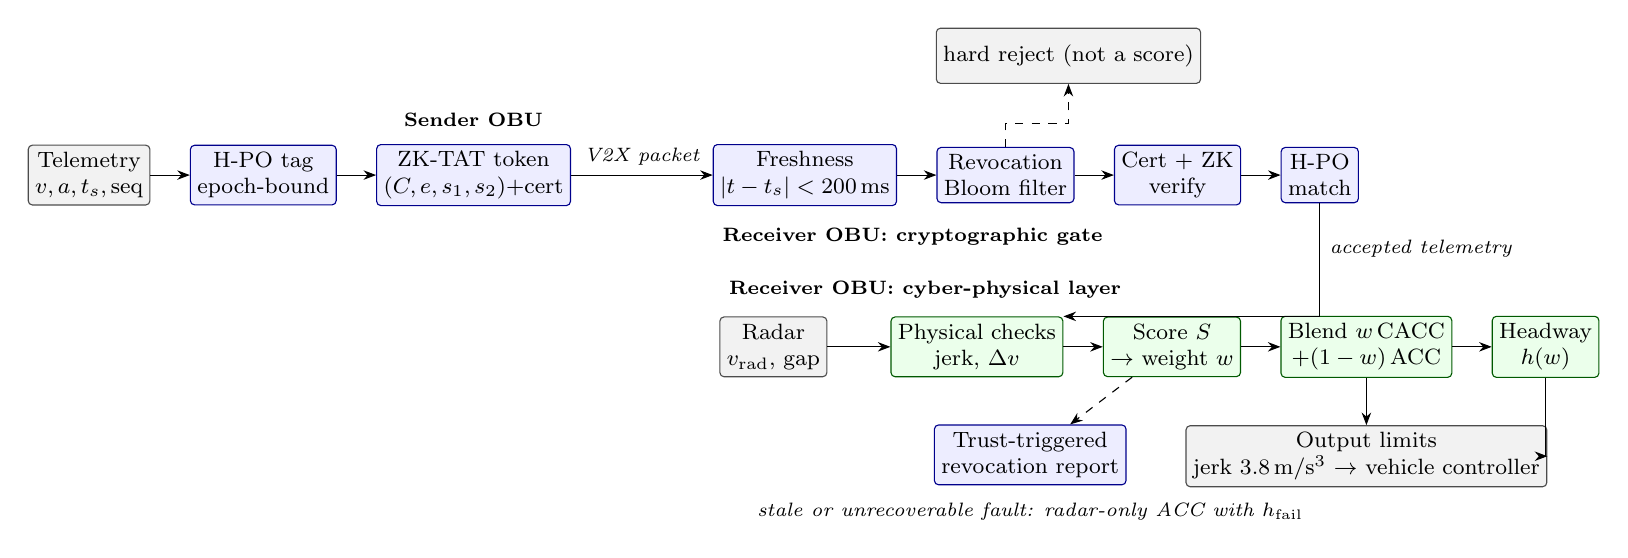
\begin{tikzpicture}[node distance=4mm and 5mm]
\node[io] (tel) {Telemetry\\$v,a,t_s,\mathrm{seq}$};
\node[cry,right=of tel] (tag) {H-PO tag\\epoch-bound};
\node[cry,right=of tag] (tok) {ZK-TAT token\\$(C,e,s_1,s_2)$+cert};
\draw[arr](tel)--(tag);\draw[arr](tag)--(tok);
\node[cry,right=18mm of tok] (f) {Freshness\\$|t-t_s|<200$\,ms};
\node[cry,right=of f] (rv) {Revocation\\Bloom filter};
\node[cry,right=of rv] (zk) {Cert + ZK\\verify};
\node[cry,right=of zk] (hp) {H-PO\\match};
\draw[arr](tok)--node[above,lab]{V2X packet}(f);
\draw[arr](f)--(rv);\draw[arr](rv)--(zk);\draw[arr](zk)--(hp);
\node[io,above=8mm of rv,xshift=8mm] (rej) {hard reject (not a score)};
\draw[arr,dashed](rv.north)--++(0,3mm)-|(rej.south);
\node[io,below=14mm of f,xshift=-4mm] (rad) {Radar\\$v_{\rm rad}$, gap};
\node[phy,right=8mm of rad] (chk) {Physical checks\\jerk, $\Delta v$};
\node[phy,right=of chk] (sc) {Score $S$\\$\to$ weight $w$};
\node[phy,right=of sc] (bl) {Blend $w\,$CACC\\$+(1-w)\,$ACC};
\node[phy,right=of bl] (hw) {Headway\\$h(w)$};
\draw[arr](rad)--(chk);\draw[arr](chk)--(sc);\draw[arr](sc)--(bl);\draw[arr](bl)--(hw);
\draw[arr](hp.south)|-node[pos=0.2,right,lab]{accepted telemetry}(chk.north east);
\node[io,below=6mm of bl] (ctl) {Output limits\\jerk 3.8\,m/s$^3$ $\to$ vehicle controller};
\draw[arr](bl)--(ctl);\draw[arr](hw.south)|-(ctl.east);
\node[cry,below=6mm of sc,xshift=-18mm] (rvk) {Trust-triggered\\revocation report};
\draw[arr,dashed](sc)--(rvk);
\node[font=\scriptsize\itshape,below=1mm of rvk,align=center] {stale or unrecoverable fault: radar-only ACC with $h_{\rm fail}$};
\node[above=1mm of tok,font=\scriptsize\bfseries] {Sender OBU};
\node[above=1mm of f,anchor=south west,xshift=-5mm,yshift=0mm,font=\scriptsize\bfseries] at (f.north west) {};
\node[font=\scriptsize\bfseries,anchor=north west] at ($(f.south west)+(0,-1.5mm)$) {Receiver OBU: cryptographic gate};
\node[font=\scriptsize\bfseries,anchor=south west] at ($(rad.north west)+(0,1mm)$) {Receiver OBU: cyber-physical layer};
\end{tikzpicture}}
\caption{CyberAdapt pipeline. Blue: cryptographic components; green: cyber-physical components; grey: sensors, inputs and actuators. A cryptographic failure is a hard reject; a physical anomaly only lowers $w$.}\label{fig:arch}
\end{figure*}

\subsection{Packet format and epoch-bound policy tags (H-PO)}
A packet carries the telemetry, a policy tag, a token and, once per pseudonym period, the issuer certificate. The policy tag hides which attribute policy a message belongs to from observers who do not hold the platoon secret. For attribute string $A$ and epoch counter $E$,
\begin{equation}
\mathrm{tag}=\mathrm{SHA\text{-}256}\big(\texttt{dom}\,\|\,\ell(A)\,\|\,A\,\|\,E\,\|\,S_{\rm pl}\big),
\end{equation}
where $\ell(A)$ is the length prefix. A receiver recomputes the tag for each of its candidate attributes. Binding the epoch removes cross-epoch linkability and cross-epoch replay of tags; within an epoch the tag is deterministic, hence linkable, which is a stated limitation. A keyed construction such as HMAC~\cite{hmac} is preferable in a deployment; our implementation provides both variants (the plain hash places the secret last, so length extension does not apply) and Table~\ref{tab:cost} reports their costs.

\subsection{Token: certified pseudonym and context-bound proof (ZK-TAT)}
Let $G$ be the generator of the Ristretto255 group of prime order $q$ (a prime-order encoding of Curve25519~\cite{bernstein2012,rfc8032}) and $H$ a second generator obtained by hashing a fixed string to the group, so that $\log_G H$ is unknown. A vehicle with identity scalar $\mathrm{VID}=H_q(\text{identity})$ obtains a pseudonym $C=rG+\mathrm{VID}\,H$ (Pedersen commitment~\cite{pedersen1991}) and an RSU Schnorr signature~\cite{schnorr1991} $\sigma_C$ on $(C,\text{validity})$. For each packet it forms the context $\mathrm{ctx}=\mathrm{SHA\text{-}256}(\text{telemetry}\,\|\,t_s\,\|\,\mathrm{seq}\,\|\,\mathrm{tag})$ and a Fiat--Shamir proof~\cite{fiatshamir1986} of knowledge of the opening $(r,\mathrm{VID})$ of $C$~\cite{okamoto1992}:
\begin{align}
R&=k_1G+k_2H,\quad e=H_q(G,H,C,R,\mathrm{ctx}),\\
s_1&=k_1+er,\quad s_2=k_2+e\,\mathrm{VID}\pmod q.
\end{align}
The token is $(C,e,s_1,s_2)$, 128\,bytes. A receiver computes $R'=s_1G+s_2H-eC$ and accepts iff $e=H_q(G,H,C,R',\mathrm{ctx})$. The certificate $\sigma_C$ (64\,bytes) is verified once per pseudonym and cached. Because the proof is bound to the telemetry and tag through $\mathrm{ctx}$, it acts as a message authenticator for the holder of the opening, while $C$ remains a pseudonym: the RSU can map $C$ to an identity from its registry, so traceability is administrative and not anonymous.

\subsection{Fixed-base precomputation (SMBP-PreComp)}
The prover's multiplications by $G$ and $H$ and the verifier's $s_1G+s_2H$ use fixed bases, so tables can be computed offline. With radix $2^w$ and $b=253$ scalar bits, the table stores $\lceil b/w\rceil(2^w-1)$ points and a multiplication costs about $b/w$ additions. For $w=1$ the table is $T[i]=2^iG$ and the cost is $\approx b/2=126$ additions on average. Variable-base double-and-add costs $b$ doublings plus about $b/2$ additions. Counting a doubling as one group operation, as with a unified addition formula, gives
\begin{equation}
\text{speed-up}_{w=1}\le\frac{b+b/2}{b/2}=3,
\end{equation}
which is the classical result for fixed-base methods~\cite{bgmw1992} and is the ceiling for this technique irrespective of hardware. Storing the table in compressed form is not free: each use needs a point decompression (a modular square root); in our Python reference implementation this made the method 22 times slower than no table at all.

\subsection{Revocation list}
Revoked pseudonym identifiers are kept in a Bloom filter~\cite{bloom1970} with $m=32\,768$ bits and $k=4$ probes, sized for $n=500$ entries, i.e.\ 4\,KiB. The expected false-positive rate is $(1-e^{-kn/m})^k=1.23\times10^{-5}$. A false positive would wrongly reject a legitimate vehicle, which is why the filter is checked after the cheap freshness test and why entries are re-issued per epoch.

\subsection{Physical plausibility and anomaly score}
For each accepted packet $k$ from the predecessor, the receiver computes
\begin{align}
J_k&=\frac{|a_k-a_{k-1}|}{t_{s,k}-t_{s,k-1}},\\
\Delta v_k&=\big|v_k+a_k(t_k-t_{s,k})-v_{\rm rad}(t_k)\big|,
\end{align}
where $v_{\rm rad}$ is the radar-derived speed of the predecessor. A check passes if $J_k\le J_{\rm lim}$ and $\Delta v_k<\Delta v_{\lim}$ with $J_{\rm lim}=10.0$\,m/s$^3$ and $\Delta v_{\lim}=1.5$\,m/s. The jerk limit is the lowest value in the tested sensitivity sweep that avoids L2 false revocations and collisions while retaining detection in A1 and A3; the same scripted scenarios informed this calibration. To obtain a graded evidence value we normalise each ratio $r$ by $z=\clip\big((r-1)/(\kappa-1),0,1\big)$ with $\kappa=4$ and take $z_k=\max(z_J,z_v)$. The score is a leaky maximum,
\begin{equation}
S_k=\max\big(z_k,\ \rho\,S_{k-1}\big),\qquad \rho=0.98,
\end{equation}
so evidence rises instantly and decays over about 3.4\,s of clean packets (half-life $\ln 0.5/\ln 0.98\approx 34$ packets).

\textbf{Enhanced plausibility checks in CyberAdapt.} Radar corroboration discounts jerk evidence when the mean reported acceleration over the last 0.5\,s agrees with radar-derived acceleration within 0.7\,m/s$^2$. When consecutive accepted packet timestamps are 0.05--0.35\,s apart, kinematic self-consistency adds $z_c=\clip((I_k/1.2-1)/(\kappa-1),0,1)$, where $I_k=|a_k-(v_k-v_{k-1})/(t_{s,k}-t_{s,k-1})|$. The final anomaly evidence is $z_k=\max(z_J,z_v,z_c)$. The first check is intended to avoid penalising corroborated braking; the second detects acceleration reports inconsistent with the reported speed history.

\subsection{Trust weight, blending and dynamic headway}
The score is mapped to a weight by a normalised sigmoid
\begin{equation}
w(S)=\clip\!\left(\frac{1+e^{-\alpha\beta}}{1+e^{\alpha(S-\beta)}},\,w_{\min},\,1\right),
\end{equation}
with $\alpha=8$, $\beta=0.45$, $w_{\min}=0.05$, which equals 1 at $S=0$ and falls monotonically (Fig.~\ref{fig:map}): $w(0.2)=0.905$, $w(0.8)=0.059$, and $w(1)$ is clamped to the floor 0.05. The weight scales the cooperative term and sets the time headway,
\begin{align}
h(w)&=h_{\rm nom}+(1-w)(h_{\rm fail}-h_{\rm nom}),\\
a_{\rm cmd}&=a_{\rm ACC}\big(h(w)\big)+w\,K_{\rm ff}\,a_{\rm rep},
\end{align}
with $h_{\rm nom}=0.6$\,s, $h_{\rm fail}=1.6$\,s; at 14\,m/s and $d_0=2.5$\,m the target gap therefore moves from 10.9\,m ($w=1$) to 24.9\,m ($w=0$). This is the blend $w\,$CACC$+(1-w)\,$ACC because CACC $=$ ACC $+K_{\rm ff}a_{\rm rep}$. The ACC law is $a_{\rm ACC}=k_pe+k_d\dot e$ with $e=\text{gap}-(d_0+hv)$ and $\dot e=v_{\rm rad}-v-ha$. Two engineering details are needed in practice and are our additions: the headway changes at most $0.25$\,s per second (otherwise a jump of $h$ demands $-5$\,m/s$^2$ braking), and the output is jerk-limited to 3.8\,m/s$^3$ except in an emergency (time-to-collision below 2\,s or gap below 4\,m).
\begin{figure}[!t]\centering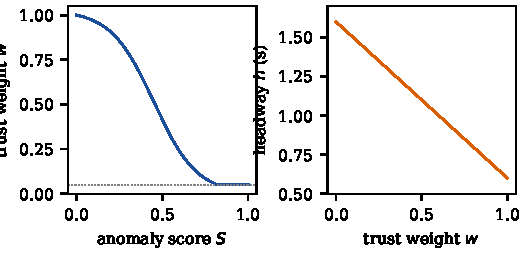
\includegraphics[width=0.8\columnwidth]{figs/mapping.pdf}
\caption{Trust weight $w(S)$ and headway $h(w)$.}\label{fig:map}\end{figure}

\subsection{Fail-safe and trust-triggered revocation}
If no valid packet arrives within $T_{\rm stale}=0.5$\,s, the vehicle sets $w=0$ and runs radar-only ACC at $h_{\rm fail}$. If $w\le0.2$ for one continuous second, the receiver reports the sender to the RSU; after a 1\,s propagation delay the sender's identifier enters the revocation filter and all receivers hard-reject it. This closes the loop between the physical and the cryptographic layer, and, as we show, it is also the riskiest part of the design.

\section{Security Analysis}\label{sec:sec}
\begin{proposition}[Completeness]An honest token for a certified $C$ with matching context is accepted.\end{proposition}
Verification computes $R'=s_1G+s_2H-eC=(k_1+er)G+(k_2+e\mathrm{VID})H-e(rG+\mathrm{VID}H)=R$.

\begin{proposition}[Soundness and hiding]In the random-oracle model, the proof is a Fiat--Shamir transform of a $\Sigma$-protocol for knowledge of a representation~\cite{okamoto1992}: two accepting transcripts with the same commitment $R$ and different challenges yield the opening of $C$, and, since $\log_GH$ is unknown, a Pedersen commitment cannot be opened two ways. $C$ is perfectly hiding, and the protocol is honest-verifier zero-knowledge.\end{proposition}
This is the standard result and is not new here.

\begin{proposition}[A proof alone authorises nothing]Without the issuer certificate, any party can generate an accepting token for an arbitrary $\mathrm{VID}'$.\end{proposition}
The prover only needs to know an opening of some $C'$ of its own choosing. With the certificate check, the sender must additionally present a signature of the RSU on $C'$, which reduces forgery to forging a Schnorr signature. We confirm both statements experimentally in Section~\ref{sec:eval}.

\begin{proposition}[Replay and context binding]A recorded packet is rejected unless it is re-sent within 200\,ms, and a token cannot be moved to different telemetry, because $e$ depends on $\mathrm{ctx}$.\end{proposition}

\begin{proposition}[Bounded influence of accepted data]\label{prop:bound}Let $a_{\rm rep}$ be clipped to $[A_{\min},A_{\max}]$ on receipt. The part of the commanded acceleration that depends on accepted V2X content is at most $w\,K_{\rm ff}\max(|A_{\min}|,A_{\max})$.\end{proposition}
This follows directly from $a_{\rm cmd}=a_{\rm ACC}(h(w))+wK_{\rm ff}a_{\rm rep}$. It does not prove collision freedom, because $a_{\rm ACC}$ also depends on $h(w)$ and on radar data; unlike~\cite{lyons2026} we give no formal safety guarantee.

\textbf{Authentic is not truthful.} A certified insider produces valid tokens for any content. The cryptographic gate therefore cannot detect A3 attacks, and Section~\ref{sec:eval} shows that a crypto-only defence behaves like no defence against them.

\textbf{Limitations of the privacy claims.} (i)~$C$ is constant over the validity period, so packets are linkable within it, as with pseudonym certificates; (ii)~H-PO tags are deterministic within an epoch; (iii)~a platoon member holding $S_{\rm pl}$ can test attribute guesses; (iv)~tracing is by RSU registry.

\section{Evaluation}\label{sec:eval}
\subsection{Implementation and simulator}
\textbf{Native implementation.} The cryptographic gate was implemented in Rust with the \texttt{curve25519-dalek} library (version 4.1.3, Ristretto255, constant-time field and point arithmetic): the fixed- and variable-base multiplications, the token, the RSU certificate, the H-PO tags with SHA-256 and HMAC-SHA-256, and the Bloom filter. Timings are means over 3000 repetitions (200\,000 for the hash and Bloom operations) on a single core of a cloud virtual machine, so absolute values will differ on an automotive OBU. An independent Python implementation over the Ed25519 prime-order subgroup was used as a cross-check and gave the same outcomes in all functional and negative tests.

\textbf{Platoon simulator.} A custom longitudinal simulator (not SUMO/Veins) models eight vehicles at 14\,m/s (the speed used in~\cite{chen2026}), a 100\,Hz control loop, first-order actuator lag ($\tau=0.1$\,s), radar at 20\,Hz (gap noise 0.05\,m, speed noise 0.05\,m/s), V2X beacons at 10\,Hz with 10--30\,ms delay and 2\% loss, and the controller of Section~\ref{sec:design} with $k_p=0.2$, $k_d=0.7$, $K_{\rm ff}=1$, $d_0=2.5$\,m, so that the nominal gap is 10.9\,m. The leader follows a $\pm1$\,m/s sinusoid. The attacker is vehicle~2 (an insider) and its target is vehicle~3. Scenarios: \textbf{L1} normal driving; \textbf{L2} severe legitimate braking of the leader at $t=30$\,s ($-6$\,m/s$^2$ reached with 15\,m/s$^3$ jerk, down to about 3\,m/s); \textbf{L3} moderate legitimate braking ($-3.5$\,m/s$^2$, 8\,m/s$^3$); \textbf{A1} false $-6$\,m/s$^2$ from $t=20$\,s; \textbf{A2} false $+3$\,m/s$^2$; \textbf{A3} acceleration-only ramp to $-3$\,m/s$^2$ at 1.5\,m/s$^3$ with truthful speed; \textbf{A4} replay at $t=60$\,s of packets recorded during the L2 braking (metrics from $t=55$\,s); \textbf{A5} forged packets without valid credentials. Each configuration is run with 20 seeds that vary noise, loss and delay. A negative minimum gap means that vehicles overlapped, i.e.\ a collision; its magnitude is not physically meaningful. The simulator models credential acceptance with flags and does not invoke the native Rust cryptographic gate, whose implementation is evaluated separately.

\textbf{Defences compared.} D0: no protection. D1: cryptographic gate only. D2: gate plus binary switch to radar-only ACC (latched for 5\,s) at $h_{\rm nom}$; D2b: the same at $h_{\rm fail}$. The binary switch triggers at $z\ge0.1$, a 30\% margin above the limit, because the unmodified threshold fired in normal operation. CyberAdapt uses the radar-corroboration and kinematic-consistency checks with $J_{\rm lim}=3$; two ablations remove revocation or the dynamic headway.

\subsection{Cryptographic cost and functional tests}
\begin{table}[!t]\centering\caption{Scalar multiplication, native Rust, Ristretto255 (mean of 3000 runs).}\label{tab:smul}\footnotesize\setlength{\tabcolsep}{2pt}
\begin{tabular}{lrrr}\toprule
Method & $\mu$s & Point additions & Speed-up\\\midrule
Double-and-add (textbook) & \natNaiveUs & $\approx$378 & 1.00\\
Fixed base, $w{=}1$ table (SMBP) & \natSmbpWUs & $\approx$126 & \natSpeedupSmbp\\
Library variable base (windowed) & \natDalekVarUs & -- & 1.88\\
Library fixed-base table & \natDalekFixedUs & -- & \natSpeedupFixedVsNaive\\\bottomrule
\end{tabular}\end{table}
Table~\ref{tab:smul} shows that our $w=1$ table (253 stored points) gives a speed-up of \natSpeedupSmbp, consistent with the bound of 3. A library's own fixed-base table, which uses a wider radix, is faster still (\natSpeedupFixedVsNaive$\times$ over the textbook method, \natSpeedupFixedVsVar$\times$ over its own windowed variable-base code). Against a modern windowed variable-base routine the gain of the simple $w=1$ table is only 1.6$\times$, so the headline ratio depends heavily on which baseline is used. We therefore report ratios against the textbook method and against the library routine separately.

\begin{table}[!t]\centering\caption{Per-packet costs (native) and sizes.}\label{tab:cost}\footnotesize\setlength{\tabcolsep}{2pt}
\begin{tabular}{lr}\toprule
Operation & Value\\\midrule
Token generation & \natZkProveUs\,$\mu$s\\
Token verification & \natZkVerifyUs\,$\mu$s (p95 \natZkVerifyP)\\
Certificate issue / verification (cached) & \natCertIssueUs\ / \natCertVerifyUs\,$\mu$s\\
H-PO tag, SHA-256 / HMAC-SHA-256 & \natHpoShaUs\ / \natHpoHmacUs\,$\mu$s\\
H-PO match, 16 candidates (HMAC) & \natHpoMatchUs\,$\mu$s\\
Bloom query ($m=32\,768$, $k=4$) & \natBloomQueryUs\,$\mu$s\\
Telemetry + tag + token & 20+32+128 = 180\,B\\
With certificate attached & 244\,B\\\bottomrule
\end{tabular}\end{table}
Table~\ref{tab:cost} lists the costs. A token verifies in about \natZkVerifyUs\,$\mu$s, i.e.\ roughly \natVerifyPerSecond\ verifications per second per core, so even verifying several neighbours at 10\,Hz uses a small fraction of a 100\,ms beacon period on this class of CPU. Packets stay within the 256\,B message size used in~\cite{chen2026}. These costs are of the same order as those of ordinary elliptic-curve signatures, which is expected, because the token is a Schnorr-type proof of knowledge.

\textbf{Functional and negative tests.} Of 300 mutated tokens per field (commitment bit flip, random $e$, $s_1$ or $s_2$, flipped context bit), none was accepted. Two proofs that reuse the same nonces on different contexts allowed the secret $r$ to be recovered by algebra, confirming that nonces must be fresh. A token generated for an uncertified random identity \emph{verified} under the proof check and was rejected by the certificate check, confirming Proposition~3. Over $2\times10^6$ non-member queries the Bloom filter gave \natBloomFp\ false positives (rate \natBloomRate$\times10^{-5}$) against a theoretical \natBloomTheory$\times10^{-5}$ (24.6 expected). H-PO tags were equal within an epoch and differed across epochs, and a wrong attribute or secret did not match.

\subsection{Platoon results}
\begin{table*}[!t]\centering\caption{Mean minimum inter-vehicle gap (m) over 20 seeds; brackets give the number of runs (out of 20) with a collision. L: legitimate scenarios, A: attacks.}\label{tab:gap}\small\setlength{\tabcolsep}{4pt}\begin{tabular}{lcccccccc}\toprule
Defence & L1 & L2 & L3 & A1 & A2 & A3 & A4 & A5\\\midrule
No protection & 10.2 & 1.3 & 6.3 & 8.2 & $-$5.9 [20] & 9.7 & 5.6 & 8.3\\
Crypto gate only & 10.2 & 1.3 & 6.3 & 8.2 & $-$5.9 [20] & 9.7 & 10.3 & 10.2\\
Binary, $h_{\rm nom}$ & 10.2 & $-$4.2 [20] & 6.3 & 8.6 & $-$5.9 [20] & 9.7 & 10.3 & 10.2\\
Binary, $h_{\rm fail}$ & 10.2 & $-$4.1 [20] & 6.3 & 9.3 & $-$6.0 [20] & 9.7 & 10.2 & 10.2\\
CyberAdapt & 10.2 & 1.2 & 6.3 & 10.1 & 9.9 & 10.1 & 10.3 & 10.2\\
\quad w/o revocation & 10.2 & 1.2 & 6.3 & 10.1 & 10.2 & 10.1 & 10.3 & 10.2\\
\quad w/o dyn.\ headway & 10.2 & 1.2 & 6.3 & 9.3 & 6.5 & 9.3 & 10.3 & 10.2\\
\bottomrule\end{tabular}\end{table*}
\textbf{Insider attacks.} Table~\ref{tab:gap} gives the central result. Against the false-acceleration insider A2, the unprotected, crypto-only and both binary-switch platoons collide in \collAtwoDzero, \collAtwoDone, \collAtwoDtwo\ and \collAtwoDtwob\ of 20 runs, whereas CyberAdapt has \collAtwoCA\ collisions and a minimum gap of \gapAtwoCA\,m (nominal 10.9\,m). Crypto-only protection is indistinguishable from no protection, as expected for an authenticated insider. The binary switch fails because the attacker's value is constant: only the onset produces a jerk spike, so the switch latches for 5\,s and then re-enables cooperative control, after which the follower is driven into its predecessor (Fig.~\ref{fig:a2}).
\begin{figure}[!t]\centering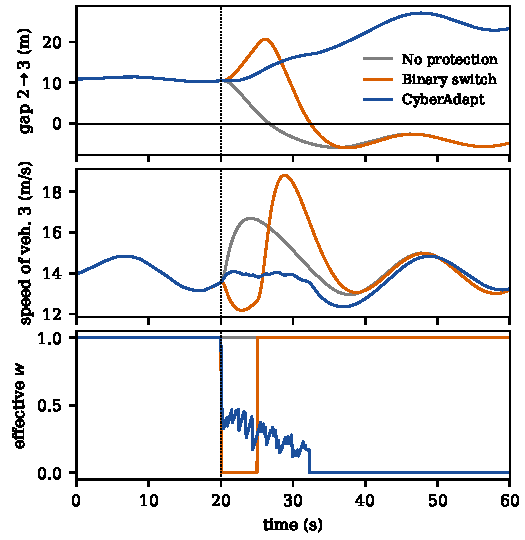
\includegraphics[width=0.95\columnwidth]{figs/a2.pdf}
\caption{Scenario A2 (false acceleration from $t=20$\,s), seed 1. The binary switch releases after 5\,s while the false value persists and the follower collides; CyberAdapt cuts the sender off and opens the gap.}\label{fig:a2}\end{figure}
\textbf{Revocation and persistent consistency evidence.} The onset of A2 raises the kinematic-consistency score because reported acceleration disagrees with reported speed change. CyberAdapt detects the attack in 20/20 runs and revokes in 20/20; without revocation, the detector still has no collisions in this scenario, with a mean minimum gap of \gapAtwoCAnr\,m versus \gapAtwoCA\,m for the full system (Table~\ref{tab:gap}). This is evidence for the checks in this scripted case, not a general safety result. The fixed-headway ablation's mean minimum gap is \gapAtwoCAfh\,m, isolating the margin contributed by dynamic headway. For false deceleration A1, the gap opens rather than closes; the minimum gap is \gapAoneDzero\,m without protection and \gapAoneCA\,m with CyberAdapt, while minimum speed is \vminAoneDzero\,m/s and \vminAoneCA\,m/s, respectively.

\textbf{Stealth.} The acceleration-only ramp A3 keeps its reported speed truthful and its jerk below the basic threshold. CyberAdapt's kinematic-consistency check detects the mismatch in all 20 runs after a mean \detAthreeCA\,s and revokes in all 20 after \revtAthreeCA\,s (Table~\ref{tab:det}). No collisions occurred in this scenario, so this experiment demonstrates detection in the modeled trace, not that the attack would cause a collision.

\textbf{Outsiders.} Forged packets (A5) reduce the minimum gap of the unprotected platoon to \gapAfiveDzero\,m and its speed to \vminAfiveDzero\,m/s, and have no effect once the gate is active (\gapAfiveDone\,m). A replay of recorded braking packets (A4) shrinks the minimum gap to \gapAfourDzero\,m without a gate and leaves \gapAfourDone\,m with one.

\begin{table}[!t]\centering\caption{Detection delay ($S>0.5$ at the receiver of the attacked sender, measured from $t=20$\,s) and trust-triggered revocation time (same origin). Counts give runs out of 20. In L2 and L3 nothing is attacked, so any entry is a false alarm; the braking starts at $t=30$\,s, i.e.\ 10\,s on this scale.}\label{tab:det}\footnotesize\setlength{\tabcolsep}{2pt}\begin{tabular}{llcc}\toprule
Scenario & Variant & Detection & Revocation\\\midrule
A1 & CyberAdapt & 0.03\,s (20/20) & 2.0\,s (20/20)\\
A2 & CyberAdapt & 0.34\,s (20/20) & 15.7\,s (20/20)\\
A3 & CyberAdapt & 1.82\,s (20/20) & 12.3\,s (20/20)\\
L2 & CyberAdapt & -- & --\\
L3 & CyberAdapt & -- & --\\
\bottomrule\end{tabular}\end{table}
\textbf{Legitimate braking and threshold sensitivity.} With the selected $J_{\rm lim}=10$\,m/s$^3$, CyberAdapt has no false revocations or collisions in the 20 L2 seeds. At the lower sensitivity settings, L2 has 6 collisions and 8 revocations at 3\,m/s$^3$ and 4 collisions with no revocations at 6\,m/s$^3$; both outcomes improve to zero at 10 and 15\,m/s$^3$ (Table~\ref{tab:jsweep}). The no-revocation ablation also has no L2 collisions at the selected setting, while both binary switches collide in all 20 runs (Table~\ref{tab:gap}, Table~\ref{tab:det}). The unified detector causes no false revocations or collisions in moderate braking L3 and preserves the unprotected mean minimum gap (\gapLthreeCA\,m). The threshold was selected using these scripted scenarios, so independent manoeuvre traces are needed before generalizing; none of these outcomes is a safety guarantee.
\begin{figure}[!t]\centering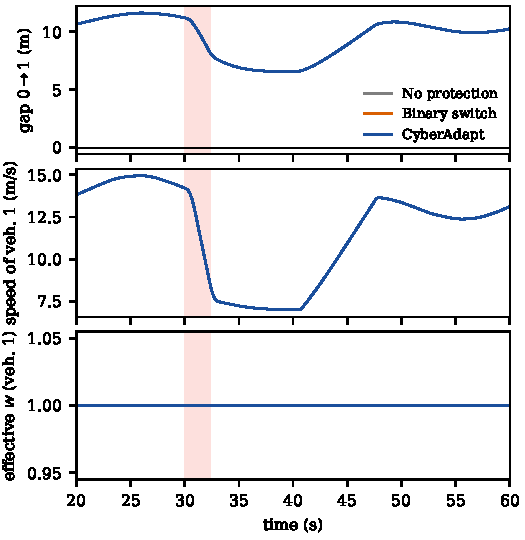
\includegraphics[width=0.95\columnwidth]{figs/l3.pdf}
\caption{Scenario L3 (legitimate moderate braking, shaded), seed 1, as seen by vehicle~1. CyberAdapt uses radar corroboration and kinematic-consistency checks to distinguish supported braking from inconsistent telemetry.}\label{fig:l3}\end{figure}
\begin{table}[!t]\centering\caption{Sensitivity to the jerk limit $J_{\rm lim}$ (CyberAdapt, 20 seeds). Min $w$ is the mean over seeds of the lowest weight seen anywhere in the platoon; Coll.: runs with a collision; Rev.: runs in which the legitimate leader was revoked.}\label{tab:jsweep}\footnotesize\setlength{\tabcolsep}{2pt}\begin{tabular}{rcccccc}\toprule
$J_{\rm lim}$ & L1 min $w$ & L2 min $w$ & L2 coll./rev. & L3 min $w$ & L3 rev. & A1 detected\\\midrule
3 & 0.94 & 0.58 & 6/8 & 0.99 & 0/20 & 20/20\\
6 & 1.00 & 0.77 & 4/0 & 1.00 & 0/20 & 20/20\\
10 & 1.00 & 0.97 & 0/0 & 1.00 & 0/20 & 20/20\\
15 & 1.00 & 1.00 & 0/0 & 1.00 & 0/20 & 20/20\\
\bottomrule\end{tabular}\end{table}
Table~\ref{tab:jsweep} shows that outcomes depend on the jerk limit. L2 has 6 collisions and 8 revocations at 3\,m/s$^3$, 4 collisions and no revocations at 6\,m/s$^3$, and no collisions or revocations at 10 or 15\,m/s$^3$. L3 has no false revocations at any tested limit, while A1 is detected in all 20 runs at each limit. A3 also remains detected in all 20 seeds at the selected 10\,m/s$^3$ limit. These outcomes depend on the braking profiles, radar and actuator model; they do not establish a universal threshold.

\begin{table}[!t]\centering\caption{Mean time gap (s) of vehicles 3--7 after $t=30$\,s (platoon efficiency; lower is better). Scenarios with a collision are marked $^\dagger$.}\label{tab:hw}\footnotesize\setlength{\tabcolsep}{2.5pt}\begin{tabular}{lcccccc}\toprule
Defence & L1 & L2 & L3 & A1 & A2 & A3\\\midrule
No protection & 0.78 & 0.85 & 0.81 & 1.21 & 0.56$^\dagger$ & 0.99\\
Crypto gate only & 0.78 & 0.85 & 0.81 & 1.21 & 0.56$^\dagger$ & 0.99\\
Binary, $h_{\rm nom}$ & 0.78 & 0.86$^\dagger$ & 0.81 & 1.21 & 0.56$^\dagger$ & 0.99\\
Binary, $h_{\rm fail}$ & 0.78 & 0.86$^\dagger$ & 0.81 & 1.21 & 0.57$^\dagger$ & 0.99\\
CyberAdapt & 0.78 & 0.85 & 0.81 & 0.98 & 0.97 & 0.98\\
\quad w/o revocation & 0.78 & 0.85 & 0.81 & 0.99 & 0.86 & 0.98\\
\quad w/o dyn.\ headway & 0.78 & 0.85 & 0.81 & 0.78 & 0.77 & 0.78\\
\bottomrule\end{tabular}\end{table}
\textbf{Efficiency and false alarms.} In normal driving (L1) CyberAdapt's minimum trust weight was at least \LoneCAminwAll\ in all runs and its trajectory matches the unprotected case; the binary switch at $h_{\rm fail}$ fired falsely in \LoneBinFalseRuns\ of 20 runs. Table~\ref{tab:hw} reports mean time gaps. In A2, CyberAdapt's mean time gap is \hwAtwoCA\,s, compared with \hwAtwoCAnr\,s without revocation and \hwAtwoCAfh\,s without dynamic headway. The dynamic headway increases the A2 minimum-gap margin from \gapAtwoCAfh\,m to \gapAtwoCA\,m, but this scripted comparison does not imply a general throughput or safety guarantee.

\subsection{Threats to validity}
The simulator is our own, with simplified radar, wireless and actuator models and no ns-3, SUMO or Veins; conclusions should be re-tested there with real traces. The scenarios are scripted, only one attacker position is studied, and parameters were chosen by the authors and varied only for $J_{\rm lim}$. The selected threshold was calibrated on these scenarios, including L2 and L3 as our design of ``legitimate hard braking''; 20 seeds vary noise, loss and delay, not scenario structure. Independent and out-of-sample validation remains necessary. Cryptographic timings come from one virtual-machine CPU, not an embedded target, and verification latency is not modelled inside the control loop.

\section{Conclusion}
CyberAdapt separates message authenticity from the question of how much an authenticated report should influence control. The unified detector combines radar corroboration with reported-acceleration/speed consistency checks. In the scripted A2 case it avoids collisions in all 20 runs, including the no-revocation ablation; it detects A3 in all runs. At the selected $J_{\rm lim}=10$\,m/s$^3$, the L2 severe-braking scenario has no false revocations or collisions in its 20 tested seeds, while L3 also has no false revocations or collisions. The L2 improvement is scenario-calibrated and does not establish collision freedom or deployment readiness. Future work should validate the plausibility limits on independent manoeuvre traces, test in SUMO/Veins with real radar and wireless traces, port the gate to an embedded target, and seek a formal safety guarantee for intermediate trust weights in the style of~\cite{lyons2026}.

\begin{thebibliography}{99}
\bibitem{chen2026}L. Chen, Y. Liu, H. Zhang, and J. Weng, ``Multi-authority attribute-based searchable encryption with attribute revocation for Internet of Vehicles,'' \emph{IEEE Trans. Veh. Technol.}, vol. 75, no. 5, pp. 8522--8533, May 2026, doi: 10.1109/TVT.2025.3629863.
\bibitem{lyons2026}L. Lyons, M. Boldrer, and L. Ferranti, ``Distributed attack-resilient platooning against false data injection,'' \emph{IEEE Trans. Veh. Technol.}, vol. 75, no. 3, pp. 3888--3903, Mar. 2026, doi: 10.1109/TVT.2025.3614452.
\bibitem{ploeg2014}J. Ploeg, N. van de Wouw, and H. Nijmeijer, ``$L_p$ string stability of cascaded systems: Application to vehicle platooning,'' \emph{IEEE Trans. Control Syst. Technol.}, vol. 22, no. 2, pp. 786--793, Mar. 2014.
\bibitem{heijden2017}R. van der Heijden, T. Lukaseder, and F. Kargl, ``Analyzing attacks on cooperative adaptive cruise control (CACC),'' in \emph{Proc. IEEE Veh. Netw. Conf.}, 2017, pp. 45--52.
\bibitem{amoozadeh2015}M. Amoozadeh \emph{et al.}, ``Security vulnerabilities of connected vehicle streams and their impact on cooperative driving,'' \emph{IEEE Commun. Mag.}, vol. 53, no. 6, pp. 126--132, Jun. 2015.
\bibitem{zhao2022}Y. Zhao, Y. Wang, X. Cheng, H. Chen, H. Yu, and Y. Ren, ``RFAP: A revocable fine-grained access control mechanism for autonomous vehicle platoon,'' \emph{IEEE Trans. Intell. Transp. Syst.}, vol. 23, no. 7, pp. 9668--9679, Jul. 2022.
\bibitem{jiang2019}F. Jiang, B. Qi, T. Wu, K. Zhu, and L. Zhang, ``CPSS: CP-ABE based platoon secure sensing scheme against cyber-attacks,'' in \emph{Proc. IEEE Intell. Transp. Syst. Conf.}, Oct. 2019, pp. 3218--3223.
\bibitem{ieee1609}\emph{IEEE Standard for Wireless Access in Vehicular Environments -- Security Services for Applications and Management Messages}, IEEE Std 1609.2-2022, 2022.
\bibitem{schnorr1991}C.-P. Schnorr, ``Efficient signature generation by smart cards,'' \emph{J. Cryptol.}, vol. 4, no. 3, pp. 161--174, 1991.
\bibitem{fiatshamir1986}A. Fiat and A. Shamir, ``How to prove yourself: Practical solutions to identification and signature problems,'' in \emph{Proc. CRYPTO}, 1986, pp. 186--194.
\bibitem{pedersen1991}T. P. Pedersen, ``Non-interactive and information-theoretic secure verifiable secret sharing,'' in \emph{Proc. CRYPTO}, 1991, pp. 129--140.
\bibitem{okamoto1992}T. Okamoto, ``Provably secure and practical identification schemes and corresponding signature schemes,'' in \emph{Proc. CRYPTO}, 1992, pp. 31--53.
\bibitem{bernstein2012}D. J. Bernstein, N. Duif, T. Lange, P. Schwabe, and B.-Y. Yang, ``High-speed high-security signatures,'' \emph{J. Cryptogr. Eng.}, vol. 2, no. 2, pp. 77--89, 2012.
\bibitem{rfc8032}S. Josefsson and I. Liusvaara, ``Edwards-curve digital signature algorithm (EdDSA),'' IETF RFC 8032, Jan. 2017.
\bibitem{bgmw1992}E. F. Brickell, D. M. Gordon, K. S. McCurley, and D. B. Wilson, ``Fast exponentiation with precomputation,'' in \emph{Proc. EUROCRYPT}, 1992, pp. 200--207.
\bibitem{bloom1970}B. H. Bloom, ``Space/time trade-offs in hash coding with allowable errors,'' \emph{Commun. ACM}, vol. 13, no. 7, pp. 422--426, Jul. 1970.
\bibitem{hmac}H. Krawczyk, M. Bellare, and R. Canetti, ``HMAC: Keyed-hashing for message authentication,'' IETF RFC 2104, Feb. 1997.
\end{thebibliography}
\end{document}
